% Created by tikzDevice version 0.12 on 2019-03-12 12:51:33
% !TEX encoding = UTF-8 Unicode
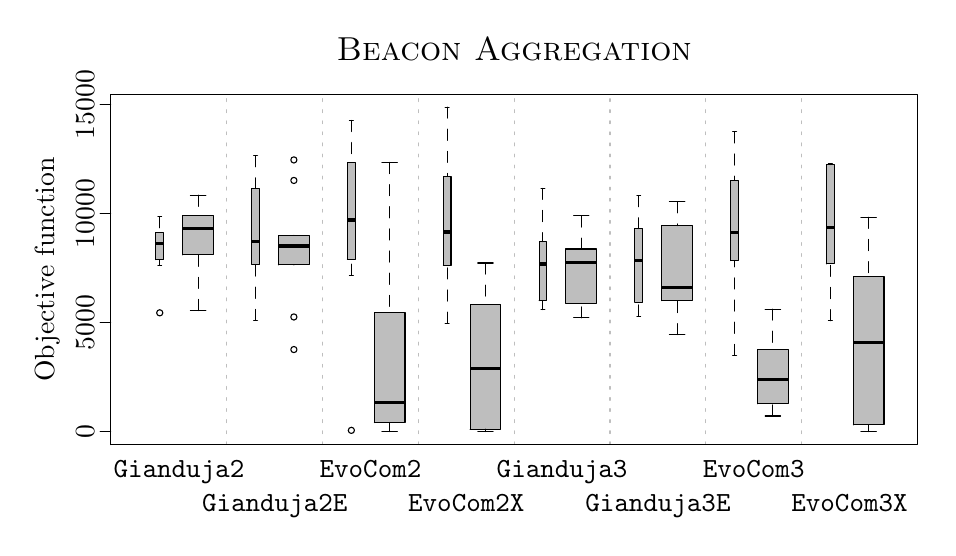
\begin{tikzpicture}[x=1pt,y=1pt]
\definecolor{fillColor}{RGB}{255,255,255}
\path[use as bounding box,fill=fillColor,fill opacity=0.00] (0,0) rectangle (325.21,180.67);
\begin{scope}
\path[clip] ( 30.00, 30.00) rectangle (321.61,156.67);
\definecolor{fillColor}{RGB}{190,190,190}

\path[fill=fillColor] ( 46.34, 96.84) --
	( 49.11, 96.84) --
	( 49.11,106.55) --
	( 46.34,106.55) --
	cycle;
\definecolor{drawColor}{RGB}{0,0,0}

\path[draw=drawColor,line width= 1.2pt,line join=round] ( 46.34,102.56) -- ( 49.11,102.56);

\path[draw=drawColor,line width= 0.4pt,dash pattern=on 4pt off 4pt ,line join=round,line cap=round] ( 47.72, 94.80) -- ( 47.72, 96.84);

\path[draw=drawColor,line width= 0.4pt,dash pattern=on 4pt off 4pt ,line join=round,line cap=round] ( 47.72,112.38) -- ( 47.72,106.55);

\path[draw=drawColor,line width= 0.4pt,line join=round,line cap=round] ( 47.03, 94.80) -- ( 48.42, 94.80);

\path[draw=drawColor,line width= 0.4pt,line join=round,line cap=round] ( 47.03,112.38) -- ( 48.42,112.38);

\path[draw=drawColor,line width= 0.4pt,line join=round,line cap=round] ( 46.34, 96.84) --
	( 49.11, 96.84) --
	( 49.11,106.55) --
	( 46.34,106.55) --
	( 46.34, 96.84);

\path[draw=drawColor,line width= 0.4pt,line join=round,line cap=round] ( 47.72, 77.63) circle (  1.12);

\path[fill=fillColor] ( 56.03, 98.57) --
	( 67.11, 98.57) --
	( 67.11,112.77) --
	( 56.03,112.77) --
	cycle;

\path[draw=drawColor,line width= 1.2pt,line join=round] ( 56.03,108.12) -- ( 67.11,108.12);

\path[draw=drawColor,line width= 0.4pt,dash pattern=on 4pt off 4pt ,line join=round,line cap=round] ( 61.57, 78.45) -- ( 61.57, 98.57);

\path[draw=drawColor,line width= 0.4pt,dash pattern=on 4pt off 4pt ,line join=round,line cap=round] ( 61.57,120.12) -- ( 61.57,112.77);

\path[draw=drawColor,line width= 0.4pt,line join=round,line cap=round] ( 58.80, 78.45) -- ( 64.34, 78.45);

\path[draw=drawColor,line width= 0.4pt,line join=round,line cap=round] ( 58.80,120.12) -- ( 64.34,120.12);

\path[draw=drawColor,line width= 0.4pt,line join=round,line cap=round] ( 56.03, 98.57) --
	( 67.11, 98.57) --
	( 67.11,112.77) --
	( 56.03,112.77) --
	( 56.03, 98.57);

\path[fill=fillColor] ( 80.96, 95.24) --
	( 83.73, 95.24) --
	( 83.73,122.70) --
	( 80.96,122.70) --
	cycle;

\path[draw=drawColor,line width= 1.2pt,line join=round] ( 80.96,103.43) -- ( 83.73,103.43);

\path[draw=drawColor,line width= 0.4pt,dash pattern=on 4pt off 4pt ,line join=round,line cap=round] ( 82.34, 74.89) -- ( 82.34, 95.24);

\path[draw=drawColor,line width= 0.4pt,dash pattern=on 4pt off 4pt ,line join=round,line cap=round] ( 82.34,134.42) -- ( 82.34,122.70);

\path[draw=drawColor,line width= 0.4pt,line join=round,line cap=round] ( 81.65, 74.89) -- ( 83.03, 74.89);

\path[draw=drawColor,line width= 0.4pt,line join=round,line cap=round] ( 81.65,134.42) -- ( 83.03,134.42);

\path[draw=drawColor,line width= 0.4pt,line join=round,line cap=round] ( 80.96, 95.24) --
	( 83.73, 95.24) --
	( 83.73,122.70) --
	( 80.96,122.70) --
	( 80.96, 95.24);

\path[fill=fillColor] ( 90.65, 94.96) --
	(101.73, 94.96) --
	(101.73,105.62) --
	( 90.65,105.62) --
	cycle;

\path[draw=drawColor,line width= 1.2pt,line join=round] ( 90.65,101.72) -- (101.73,101.72);

\path[draw=drawColor,line width= 0.4pt,dash pattern=on 4pt off 4pt ,line join=round,line cap=round] ( 96.19, 94.96) -- ( 96.19, 94.96);

\path[draw=drawColor,line width= 0.4pt,dash pattern=on 4pt off 4pt ,line join=round,line cap=round] ( 96.19,105.62) -- ( 96.19,105.62);

\path[draw=drawColor,line width= 0.4pt,line join=round,line cap=round] ( 93.42, 94.96) -- ( 98.96, 94.96);

\path[draw=drawColor,line width= 0.4pt,line join=round,line cap=round] ( 93.42,105.62) -- ( 98.96,105.62);

\path[draw=drawColor,line width= 0.4pt,line join=round,line cap=round] ( 90.65, 94.96) --
	(101.73, 94.96) --
	(101.73,105.62) --
	( 90.65,105.62) --
	( 90.65, 94.96);

\path[draw=drawColor,line width= 0.4pt,line join=round,line cap=round] ( 96.19,132.88) circle (  1.12);

\path[draw=drawColor,line width= 0.4pt,line join=round,line cap=round] ( 96.19, 64.36) circle (  1.12);

\path[draw=drawColor,line width= 0.4pt,line join=round,line cap=round] ( 96.19,125.46) circle (  1.12);

\path[draw=drawColor,line width= 0.4pt,line join=round,line cap=round] ( 96.19, 76.13) circle (  1.12);

\path[fill=fillColor] (115.57, 96.96) --
	(118.34, 96.96) --
	(118.34,131.90) --
	(115.57,131.90) --
	cycle;

\path[draw=drawColor,line width= 1.2pt,line join=round] (115.57,111.19) -- (118.34,111.19);

\path[draw=drawColor,line width= 0.4pt,dash pattern=on 4pt off 4pt ,line join=round,line cap=round] (116.96, 91.21) -- (116.96, 96.96);

\path[draw=drawColor,line width= 0.4pt,dash pattern=on 4pt off 4pt ,line join=round,line cap=round] (116.96,147.16) -- (116.96,131.90);

\path[draw=drawColor,line width= 0.4pt,line join=round,line cap=round] (116.27, 91.21) -- (117.65, 91.21);

\path[draw=drawColor,line width= 0.4pt,line join=round,line cap=round] (116.27,147.16) -- (117.65,147.16);

\path[draw=drawColor,line width= 0.4pt,line join=round,line cap=round] (115.57, 96.96) --
	(118.34, 96.96) --
	(118.34,131.90) --
	(115.57,131.90) --
	(115.57, 96.96);

\path[draw=drawColor,line width= 0.4pt,line join=round,line cap=round] (116.96, 35.16) circle (  1.12);

\path[fill=fillColor] (125.27, 37.98) --
	(136.34, 37.98) --
	(136.34, 77.70) --
	(125.27, 77.70) --
	cycle;

\path[draw=drawColor,line width= 1.2pt,line join=round] (125.27, 45.16) -- (136.34, 45.16);

\path[draw=drawColor,line width= 0.4pt,dash pattern=on 4pt off 4pt ,line join=round,line cap=round] (130.81, 34.69) -- (130.81, 37.98);

\path[draw=drawColor,line width= 0.4pt,dash pattern=on 4pt off 4pt ,line join=round,line cap=round] (130.81,131.96) -- (130.81, 77.70);

\path[draw=drawColor,line width= 0.4pt,line join=round,line cap=round] (128.04, 34.69) -- (133.57, 34.69);

\path[draw=drawColor,line width= 0.4pt,line join=round,line cap=round] (128.04,131.96) -- (133.57,131.96);

\path[draw=drawColor,line width= 0.4pt,line join=round,line cap=round] (125.27, 37.98) --
	(136.34, 37.98) --
	(136.34, 77.70) --
	(125.27, 77.70) --
	(125.27, 37.98);

\path[fill=fillColor] (150.19, 94.80) --
	(152.96, 94.80) --
	(152.96,126.99) --
	(150.19,126.99) --
	cycle;

\path[draw=drawColor,line width= 1.2pt,line join=round] (150.19,106.86) -- (152.96,106.86);

\path[draw=drawColor,line width= 0.4pt,dash pattern=on 4pt off 4pt ,line join=round,line cap=round] (151.58, 73.87) -- (151.58, 94.80);

\path[draw=drawColor,line width= 0.4pt,dash pattern=on 4pt off 4pt ,line join=round,line cap=round] (151.58,151.98) -- (151.58,126.99);

\path[draw=drawColor,line width= 0.4pt,line join=round,line cap=round] (150.88, 73.87) -- (152.27, 73.87);

\path[draw=drawColor,line width= 0.4pt,line join=round,line cap=round] (150.88,151.98) -- (152.27,151.98);

\path[draw=drawColor,line width= 0.4pt,line join=round,line cap=round] (150.19, 94.80) --
	(152.96, 94.80) --
	(152.96,126.99) --
	(150.19,126.99) --
	(150.19, 94.80);

\path[fill=fillColor] (159.88, 35.61) --
	(170.96, 35.61) --
	(170.96, 80.78) --
	(159.88, 80.78) --
	cycle;

\path[draw=drawColor,line width= 1.2pt,line join=round] (159.88, 57.51) -- (170.96, 57.51);

\path[draw=drawColor,line width= 0.4pt,dash pattern=on 4pt off 4pt ,line join=round,line cap=round] (165.42, 34.69) -- (165.42, 35.61);

\path[draw=drawColor,line width= 0.4pt,dash pattern=on 4pt off 4pt ,line join=round,line cap=round] (165.42, 95.65) -- (165.42, 80.78);

\path[draw=drawColor,line width= 0.4pt,line join=round,line cap=round] (162.65, 34.69) -- (168.19, 34.69);

\path[draw=drawColor,line width= 0.4pt,line join=round,line cap=round] (162.65, 95.65) -- (168.19, 95.65);

\path[draw=drawColor,line width= 0.4pt,line join=round,line cap=round] (159.88, 35.61) --
	(170.96, 35.61) --
	(170.96, 80.78) --
	(159.88, 80.78) --
	(159.88, 35.61);

\path[fill=fillColor] (184.81, 82.06) --
	(187.58, 82.06) --
	(187.58,103.34) --
	(184.81,103.34) --
	cycle;

\path[draw=drawColor,line width= 1.2pt,line join=round] (184.81, 95.26) -- (187.58, 95.26);

\path[draw=drawColor,line width= 0.4pt,dash pattern=on 4pt off 4pt ,line join=round,line cap=round] (186.19, 78.78) -- (186.19, 82.06);

\path[draw=drawColor,line width= 0.4pt,dash pattern=on 4pt off 4pt ,line join=round,line cap=round] (186.19,122.61) -- (186.19,103.34);

\path[draw=drawColor,line width= 0.4pt,line join=round,line cap=round] (185.50, 78.78) -- (186.88, 78.78);

\path[draw=drawColor,line width= 0.4pt,line join=round,line cap=round] (185.50,122.61) -- (186.88,122.61);

\path[draw=drawColor,line width= 0.4pt,line join=round,line cap=round] (184.81, 82.06) --
	(187.58, 82.06) --
	(187.58,103.34) --
	(184.81,103.34) --
	(184.81, 82.06);

\path[fill=fillColor] (194.50, 81.02) --
	(205.58, 81.02) --
	(205.58,100.70) --
	(194.50,100.70) --
	cycle;

\path[draw=drawColor,line width= 1.2pt,line join=round] (194.50, 95.70) -- (205.58, 95.70);

\path[draw=drawColor,line width= 0.4pt,dash pattern=on 4pt off 4pt ,line join=round,line cap=round] (200.04, 75.80) -- (200.04, 81.02);

\path[draw=drawColor,line width= 0.4pt,dash pattern=on 4pt off 4pt ,line join=round,line cap=round] (200.04,112.64) -- (200.04,100.70);

\path[draw=drawColor,line width= 0.4pt,line join=round,line cap=round] (197.27, 75.80) -- (202.81, 75.80);

\path[draw=drawColor,line width= 0.4pt,line join=round,line cap=round] (197.27,112.64) -- (202.81,112.64);

\path[draw=drawColor,line width= 0.4pt,line join=round,line cap=round] (194.50, 81.02) --
	(205.58, 81.02) --
	(205.58,100.70) --
	(194.50,100.70) --
	(194.50, 81.02);

\path[fill=fillColor] (219.43, 81.49) --
	(222.19, 81.49) --
	(222.19,108.10) --
	(219.43,108.10) --
	cycle;

\path[draw=drawColor,line width= 1.2pt,line join=round] (219.43, 96.56) -- (222.19, 96.56);

\path[draw=drawColor,line width= 0.4pt,dash pattern=on 4pt off 4pt ,line join=round,line cap=round] (220.81, 76.45) -- (220.81, 81.49);

\path[draw=drawColor,line width= 0.4pt,dash pattern=on 4pt off 4pt ,line join=round,line cap=round] (220.81,119.97) -- (220.81,108.10);

\path[draw=drawColor,line width= 0.4pt,line join=round,line cap=round] (220.12, 76.45) -- (221.50, 76.45);

\path[draw=drawColor,line width= 0.4pt,line join=round,line cap=round] (220.12,119.97) -- (221.50,119.97);

\path[draw=drawColor,line width= 0.4pt,line join=round,line cap=round] (219.43, 81.49) --
	(222.19, 81.49) --
	(222.19,108.10) --
	(219.43,108.10) --
	(219.43, 81.49);

\path[fill=fillColor] (229.12, 82.05) --
	(240.20, 82.05) --
	(240.20,109.15) --
	(229.12,109.15) --
	cycle;

\path[draw=drawColor,line width= 1.2pt,line join=round] (229.12, 86.86) -- (240.20, 86.86);

\path[draw=drawColor,line width= 0.4pt,dash pattern=on 4pt off 4pt ,line join=round,line cap=round] (234.66, 69.75) -- (234.66, 82.05);

\path[draw=drawColor,line width= 0.4pt,dash pattern=on 4pt off 4pt ,line join=round,line cap=round] (234.66,117.74) -- (234.66,109.15);

\path[draw=drawColor,line width= 0.4pt,line join=round,line cap=round] (231.89, 69.75) -- (237.43, 69.75);

\path[draw=drawColor,line width= 0.4pt,line join=round,line cap=round] (231.89,117.74) -- (237.43,117.74);

\path[draw=drawColor,line width= 0.4pt,line join=round,line cap=round] (229.12, 82.05) --
	(240.20, 82.05) --
	(240.20,109.15) --
	(229.12,109.15) --
	(229.12, 82.05);

\path[fill=fillColor] (254.04, 96.49) --
	(256.81, 96.49) --
	(256.81,125.49) --
	(254.04,125.49) --
	cycle;

\path[draw=drawColor,line width= 1.2pt,line join=round] (254.04,106.70) -- (256.81,106.70);

\path[draw=drawColor,line width= 0.4pt,dash pattern=on 4pt off 4pt ,line join=round,line cap=round] (255.43, 62.25) -- (255.43, 96.49);

\path[draw=drawColor,line width= 0.4pt,dash pattern=on 4pt off 4pt ,line join=round,line cap=round] (255.43,143.01) -- (255.43,125.49);

\path[draw=drawColor,line width= 0.4pt,line join=round,line cap=round] (254.73, 62.25) -- (256.12, 62.25);

\path[draw=drawColor,line width= 0.4pt,line join=round,line cap=round] (254.73,143.01) -- (256.12,143.01);

\path[draw=drawColor,line width= 0.4pt,line join=round,line cap=round] (254.04, 96.49) --
	(256.81, 96.49) --
	(256.81,125.49) --
	(254.04,125.49) --
	(254.04, 96.49);

\path[fill=fillColor] (263.74, 44.79) --
	(274.81, 44.79) --
	(274.81, 64.30) --
	(263.74, 64.30) --
	cycle;

\path[draw=drawColor,line width= 1.2pt,line join=round] (263.74, 53.45) -- (274.81, 53.45);

\path[draw=drawColor,line width= 0.4pt,dash pattern=on 4pt off 4pt ,line join=round,line cap=round] (269.27, 40.35) -- (269.27, 44.79);

\path[draw=drawColor,line width= 0.4pt,dash pattern=on 4pt off 4pt ,line join=round,line cap=round] (269.27, 78.99) -- (269.27, 64.30);

\path[draw=drawColor,line width= 0.4pt,line join=round,line cap=round] (266.50, 40.35) -- (272.04, 40.35);

\path[draw=drawColor,line width= 0.4pt,line join=round,line cap=round] (266.50, 78.99) -- (272.04, 78.99);

\path[draw=drawColor,line width= 0.4pt,line join=round,line cap=round] (263.74, 44.79) --
	(274.81, 44.79) --
	(274.81, 64.30) --
	(263.74, 64.30) --
	(263.74, 44.79);

\path[fill=fillColor] (288.66, 95.35) --
	(291.43, 95.35) --
	(291.43,131.24) --
	(288.66,131.24) --
	cycle;

\path[draw=drawColor,line width= 1.2pt,line join=round] (288.66,108.49) -- (291.43,108.49);

\path[draw=drawColor,line width= 0.4pt,dash pattern=on 4pt off 4pt ,line join=round,line cap=round] (290.04, 74.78) -- (290.04, 95.35);

\path[draw=drawColor,line width= 0.4pt,dash pattern=on 4pt off 4pt ,line join=round,line cap=round] (290.04,131.48) -- (290.04,131.24);

\path[draw=drawColor,line width= 0.4pt,line join=round,line cap=round] (289.35, 74.78) -- (290.74, 74.78);

\path[draw=drawColor,line width= 0.4pt,line join=round,line cap=round] (289.35,131.48) -- (290.74,131.48);

\path[draw=drawColor,line width= 0.4pt,line join=round,line cap=round] (288.66, 95.35) --
	(291.43, 95.35) --
	(291.43,131.24) --
	(288.66,131.24) --
	(288.66, 95.35);

\path[fill=fillColor] (298.35, 37.13) --
	(309.43, 37.13) --
	(309.43, 90.90) --
	(298.35, 90.90) --
	cycle;

\path[draw=drawColor,line width= 1.2pt,line join=round] (298.35, 66.82) -- (309.43, 66.82);

\path[draw=drawColor,line width= 0.4pt,dash pattern=on 4pt off 4pt ,line join=round,line cap=round] (303.89, 34.69) -- (303.89, 37.13);

\path[draw=drawColor,line width= 0.4pt,dash pattern=on 4pt off 4pt ,line join=round,line cap=round] (303.89,112.15) -- (303.89, 90.90);

\path[draw=drawColor,line width= 0.4pt,line join=round,line cap=round] (301.12, 34.69) -- (306.66, 34.69);

\path[draw=drawColor,line width= 0.4pt,line join=round,line cap=round] (301.12,112.15) -- (306.66,112.15);

\path[draw=drawColor,line width= 0.4pt,line join=round,line cap=round] (298.35, 37.13) --
	(309.43, 37.13) --
	(309.43, 90.90) --
	(298.35, 90.90) --
	(298.35, 37.13);
\definecolor{drawColor}{RGB}{190,190,190}

\path[draw=drawColor,line width= 0.4pt,dash pattern=on 1pt off 3pt ,line join=round,line cap=round] ( 71.96, 30.00) -- ( 71.96,156.67);

\path[draw=drawColor,line width= 0.4pt,dash pattern=on 1pt off 3pt ,line join=round,line cap=round] (106.57, 30.00) -- (106.57,156.67);

\path[draw=drawColor,line width= 0.4pt,dash pattern=on 1pt off 3pt ,line join=round,line cap=round] (141.19, 30.00) -- (141.19,156.67);

\path[draw=drawColor,line width= 0.4pt,dash pattern=on 1pt off 3pt ,line join=round,line cap=round] (175.81, 30.00) -- (175.81,156.67);

\path[draw=drawColor,line width= 0.4pt,dash pattern=on 1pt off 3pt ,line join=round,line cap=round] (210.42, 30.00) -- (210.42,156.67);

\path[draw=drawColor,line width= 0.4pt,dash pattern=on 1pt off 3pt ,line join=round,line cap=round] (245.04, 30.00) -- (245.04,156.67);

\path[draw=drawColor,line width= 0.4pt,dash pattern=on 1pt off 3pt ,line join=round,line cap=round] (279.66, 30.00) -- (279.66,156.67);
\end{scope}
\begin{scope}
\path[clip] (  0.00,  0.00) rectangle (325.21,180.67);
\definecolor{drawColor}{RGB}{0,0,0}

\node[text=drawColor,anchor=base,inner sep=0pt, outer sep=0pt, scale=  1.00] at ( 54.65, 18.00) {\texttt{Gianduja2}};

\node[text=drawColor,anchor=base,inner sep=0pt, outer sep=0pt, scale=  1.00] at (123.88, 18.00) {\texttt{EvoCom2}};

\node[text=drawColor,anchor=base,inner sep=0pt, outer sep=0pt, scale=  1.00] at (193.12, 18.00) {\texttt{Gianduja3}};

\node[text=drawColor,anchor=base,inner sep=0pt, outer sep=0pt, scale=  1.00] at (262.35, 18.00) {\texttt{EvoCom3}};

\node[text=drawColor,anchor=base,inner sep=0pt, outer sep=0pt, scale=  1.00] at ( 89.26,  6.00) {\texttt{Gianduja2E}};

\node[text=drawColor,anchor=base,inner sep=0pt, outer sep=0pt, scale=  1.00] at (158.50,  6.00) {\texttt{EvoCom2X}};

\node[text=drawColor,anchor=base,inner sep=0pt, outer sep=0pt, scale=  1.00] at (227.73,  6.00) {\texttt{Gianduja3E}};

\node[text=drawColor,anchor=base,inner sep=0pt, outer sep=0pt, scale=  1.00] at (296.97,  6.00) {\texttt{EvoCom3X}};
\end{scope}
\begin{scope}
\path[clip] (  0.00,  0.00) rectangle (325.21,180.67);
\definecolor{drawColor}{RGB}{0,0,0}

\node[text=drawColor,anchor=base,inner sep=0pt, outer sep=0pt, scale=  1.20] at (175.81,168.67) {\textsc{Beacon Aggregation}};

\node[text=drawColor,rotate= 90.00,anchor=base,inner sep=0pt, outer sep=0pt, scale=  1.00] at (  9.60, 93.34) {Objective function};
\end{scope}
\begin{scope}
\path[clip] (  0.00,  0.00) rectangle (325.21,180.67);
\definecolor{drawColor}{RGB}{0,0,0}

\path[draw=drawColor,line width= 0.4pt,line join=round,line cap=round] ( 30.00, 34.68) -- ( 30.00,152.87);

\path[draw=drawColor,line width= 0.4pt,line join=round,line cap=round] ( 30.00, 34.68) -- ( 26.20, 34.68);

\path[draw=drawColor,line width= 0.4pt,line join=round,line cap=round] ( 30.00, 74.08) -- ( 26.20, 74.08);

\path[draw=drawColor,line width= 0.4pt,line join=round,line cap=round] ( 30.00,113.48) -- ( 26.20,113.48);

\path[draw=drawColor,line width= 0.4pt,line join=round,line cap=round] ( 30.00,152.87) -- ( 26.20,152.87);

\node[text=drawColor,rotate= 90.00,anchor=base,inner sep=0pt, outer sep=0pt, scale=  1.00] at ( 24.00, 34.68) {0};

\node[text=drawColor,rotate= 90.00,anchor=base,inner sep=0pt, outer sep=0pt, scale=  1.00] at ( 24.00, 74.08) {5000};

\node[text=drawColor,rotate= 90.00,anchor=base,inner sep=0pt, outer sep=0pt, scale=  1.00] at ( 24.00,113.48) {10000};

\node[text=drawColor,rotate= 90.00,anchor=base,inner sep=0pt, outer sep=0pt, scale=  1.00] at ( 24.00,152.87) {15000};

\path[draw=drawColor,line width= 0.4pt,line join=round,line cap=round] ( 30.00, 30.00) --
	(321.61, 30.00) --
	(321.61,156.67) --
	( 30.00,156.67) --
	( 30.00, 30.00);
\end{scope}
\end{tikzpicture}
